\documentclass[a4paper,14pt]{article}
\usepackage{float}
\usepackage{extsizes}
\usepackage{amsmath}
\usepackage{amssymb}
\everymath{\displaystyle}
\usepackage{geometry}
\usepackage{fancyhdr}
\usepackage{multicol}
\usepackage{graphicx}
\usepackage[brazil]{babel}
\usepackage[shortlabels]{enumitem}
\usepackage{cancel}
\usepackage{textcomp}
\usepackage{array} % Para melhor formatação de tabelas
\usepackage{longtable}
\usepackage{booktabs}  % Para linhas horizontais mais bonitas
\usepackage{float}   % Para usar o modificador [H]
\usepackage{caption} % Para usar legendas em tabelas
\usepackage{tcolorbox}

\columnsep=2cm
\hoffset=0cm
\textwidth=8cm
\setlength{\columnseprule}{.1pt}
\setlength{\columnsep}{2cm}
\renewcommand{\headrulewidth}{0pt}
\geometry{top=1in, bottom=1in, left=0.7in, right=0.5in}

\pagestyle{fancy}
\fancyhf{}
\fancyfoot[C]{\thepage}

\begin{document}
	
	\noindent\textbf{6FMA41 - Matemática} 
	
	\begin{center}Descrevendo situações com adição de inteiros (Versão estudante)
	\end{center}
	
	\noindent\textbf{Nome:} \underline{\hspace{10cm}}
	\noindent\textbf{Data:} \underline{\hspace{4cm}}
	
	%\section*{Questões de Matemática}
	\begin{multicols}{2}
		\noindent Nesta aula, descrevemos algumas situações utilizando a adição de números inteiros.
	\textsubscript{---------------------------------------------------------------------}
    	\begin{enumerate}
    		\item Na reta abaixo está desenhado $x$. Se eu "andar" para a direita 8 unidades, como descrever a nova situação? \\
    		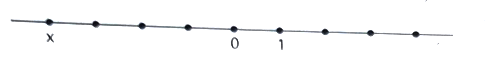
\includegraphics[width=1\linewidth]{6FMA41_imagens/imagem1} \\\\
    		\item Manoel tinha saldo de -150 reais no banco. Sacou do caixa eletrônico 200 reais.
    		\begin{enumerate}[a)]
    			\item Descreva, usando adição, o saldo atual de Manoel. \\\\\\
    			\item Qual é o saldo atual de Manoel? \\\\\\
    		\end{enumerate}
    		\item Marcelo joga uma partida de figurinhas e perde 3 figurinhas. Joga outra e perde 6.
    		\begin{enumerate}[a)]
    			\item Como descrever, usando adição, as partidas anteriores? \\\\
    			\item Quantas figurinhas ele ganhou ou perdeu no final? \\\\\\\\\\
    		\end{enumerate}
    		\item Uma pessoa fez duas semanas de regime. Na primeira semana, perdeu 3 quilogramas. Na segunda semana, perdeu 4 quilogramas.
    		\begin{enumerate}[a)]
    			\item Descreva, usando adição, quantos quilogramas essa pessoa ganhou ou perdeu nas duas semanas. \\\\\\
    			\item Quantos quilogramas essa pessoa ganhou ou perdeu? \\\\\\
    		\end{enumerate}
    		\item \begin{enumerate}[a)]
    			\item Pedro é 15 cm mais baixo que André. André tem $a$ cm. Descreva, usando adição, a altura de Pedro. \\\\\\\\\\
    			\item Caso pedro fosse 12 cm mais alto que André, qual seria a altura de Pedro? Utilize a adição para descrevê-la. \\\\\\\\\\
    		\end{enumerate}
    		\item \begin{enumerate}[a)]
    			\item João é 12 cm mais alto que José. José tem $b$ cm. Descreva, usando adição, a altura de João. \\\\\\\\\\
    			\item Complete o enunciado seguindo o modelo do item anterior e responda-o: \\
    			Fernanda é \underline{~~~~~~~~} cm mais \underline{~~~~~~~~} que sua irmã, que tem $x$ cm. Descreva, usando adição, a altura de Fernanda.
    		\end{enumerate}
    	\end{enumerate}
    	$~$ \\ $~$ \\ $~$ \\ $~$ \\ $~$ \\ $~$ \\ $~$ \\ $~$ \\ $~$ \\ $~$ \\ $~$ \\ $~$ \\ $~$ \\ $~$ \\ $~$ \\ $~$ \\ $~$ \\ $~$ \\ $~$ \\ $~$ \\ $~$ \\ $~$ \\ $~$ \\ $~$ \\ $~$ \\ $~$ \\ $~$ \\ $~$ \\ $~$ \\ $~$ \\ $~$ \\ $~$ \\ $~$ \\ $~$ \\ $~$ \\ $~$ \\ $~$ \\ $~$ \\ $~$ \\ $~$ \\ $~$ \\ $~$ \\ $~$ \\ $~$ \\ $~$ \\ $~$ \\ $~$ \\ $~$ \\ $~$ \\ $~$ \\ $~$ \\ $~$ \\ $~$ \\ $~$ \\ $~$ \\ $~$ \\
	\end{multicols}
\end{document}